%%% Для сборки выполнить 2 раза команду: pdflatex <имя файла>

\documentclass[a4paper,12pt]{article}

\usepackage{ucs}
\usepackage[utf8x]{inputenc}
\usepackage[russian]{babel}
%\usepackage{cmlgc}
\usepackage{graphicx}
\usepackage{listings}
\usepackage{xcolor}
\usepackage{titlesec}
%\usepackage{courier}

\makeatletter
\renewcommand\@biblabel[1]{#1.}
\makeatother

\newcommand{\myrule}[1]{\rule{#1}{0.4pt}}
\newcommand{\sign}[2][~]{{\small\myrule{#2}\\[-0.7em]\makebox[#2]{\it #1}}}

% Поля
\usepackage[top=20mm, left=30mm, right=10mm, bottom=20mm, nohead]{geometry}
\usepackage{indentfirst}

% Межстрочный интервал
\renewcommand{\baselinestretch}{1.50}

% ------------------------------------------------------------------------------
% minted
% ------------------------------------------------------------------------------
% \usepackage{minted}


% ------------------------------------------------------------------------------
% tcolorbox / tcblisting
% ------------------------------------------------------------------------------

%%%%%%%%%%%%%%%%%%%%%%%%%%%%%%%%%%%%%%%

\begin{document}

%%%%%%%%%%%%%%%%%%%%%%%%%%%%%%%
%%%                         %%%
%%% Начало титульного листа %%%

\thispagestyle{empty}
\begin{center}


    \renewcommand{\baselinestretch}{1}
    {\large
        {\sc Петрозаводский государственный университет\\
            Институт математики и информационных технологий\\
            Кафедра информатики и математического обеспечения
        }
    }

\end{center}


\begin{center}
    %%%%%%%%%%%%%%%%%%%%%%%%%
    %
    % Раскомментируйте (уберите знак процента в начале строки)
    % для одной из строк типа направления  - бакалавриат/
    % магистратура и для одной из
    % строк Вашего направление подготовки
    %
    Направление подготовки бакалавриата \\
    % 01.03.02 --- Прикладная математика и информатика \\
    % 09.03.02 --- Информационные системы и технологии \\
    09.03.04 --- Программная инженерия \\
    %%%%%%%%%%%%%%%%%%%%%%%%%
\end{center}

\vfill

\begin{center}
    {\normalsize
    Отчет о проектной работе по курсу <<Разработка приложений для мобильных ОС>>}

    \medskip

    %%% Название работы %%%
    {\Large \sc {Приложение <<TODO>> }} \\
\end{center}

\medskip

\begin{flushright}
    \parbox{11cm}{%
        \renewcommand{\baselinestretch}{1.2}
        \normalsize
        Выполнил:\\
        % Выполнили:\\
        Куусела Демид Александрович\\
        %%% ФИО студента %%%
        студент 2 курса группы 22207
        \begin{flushright}
            Д. А. Куусела \sign[подпись]{4cm}
        \end{flushright}

        %%% Второй участник %%%
        % студента 1 курса группы 2210X
        % \begin{flushright}
        % 	И. О. Фамилия \sign[подпись]{4cm}
        % \end{flushright}

        %%%%%%%%%%%%%%%%%%%%%%%%%
        % девушкам применять "Выполнила" и "студентка"
        %%%%%%%%%%%%%%%%%%%%%%%%%
    }
\end{flushright}

\vfill

\begin{center}
    \large
    Петрозаводск --- 2021
\end{center}

%%% Конец титульного листа  %%%
%%%                         %%%
%%%%%%%%%%%%%%%%%%%%%%%%%%%%%%%

%%%%%%%%%%%%%%%%%%%%%%%%%%%%%%%%
%%%                          %%%
%%% Содержание               %%%

\newpage

\tableofcontents

%%% Содержание              %%%
%%%                         %%%
%%%%%%%%%%%%%%%%%%%%%%%%%%%%%%%

%%%%%%%%%%%%%%%%%%%%%%%%%%%%%%%%
%%%                          %%%
%%% Введение                 %%%

%%% В введении Вы должны описать предметную область, с которой связана %%%
%%% Ваша работа, показать её актуальность, вкратце определить цель     %%%
%%% разработки					       %%%


\newpage
\section*{Введение}
\addcontentsline{toc}{section}{Введение}

Цель проекта: разработать мобильное приложение для управления задач.

Задачи проекта:
\begin{enumerate}
    \item Организовать хранение данных о задачах
    \item Организовать хранение данных о задачах при выключенном приложении
    \item Разработать интерфейс приложения
    \item Разработать функции для загрузки информации в главный фрагмент
\end{enumerate}

%%%                          %%%
%%%%%%%%%%%%%%%%%%%%%%%%%%%%%%%%

%%%%%%%%%%%%%%%%%%%%%%%%%%%%%%%
%%% Требования к приложению %%%
% \newpage
\section{Требования к приложению}
\begin{enumerate}
    \item Возможность просматривать текущие задачи
    \item Возможность добавлять новые задачи
    \item Возможность удалять задачи
\end{enumerate}
% \subsection{Подраздел}

%%%                                     %%%
%%%%%%%%%%%%%%%%%%%%%%%%%%%%%%%%%%%%%%%%%%%

%%%%%%%%%%%%%%%%%%%%%%%%%%%%%%%%%%%%%%%%%%%
%%%                                     %%%
%%% Проектирование приложения           %%%
% \newpage
\section{Проектирование приложения}
\subsection{MainActivity.kt}
Главный Kotlin файл, создаёт и запускает Activity.
\subsection{MainFragment.kt}
Kotlin файл, подгружает данные с помощью функции loadTasks, навешивает "прослушку" на кнопку добавления новой задачи. Также в MainFragment есть несколько функций:
\begin{itemize}
    \item addTask --- преобразование содержимого поля ввода в строку, добавление новой задачи в список, очищение поля ввода;
    \item saveTasks --- сохранение текущих задач в SharedPreferences;
    \item loadTasks --- подгрузка данных из SharedPreferences.  
\end{itemize}
\subsection{CustomAdapter.kt}
Kotlin файл, адаптер между моделью и отображением (view). Функции:
\begin{itemize}
    \item addTask --- добавление задачи в модель и вызов сохранения данных;
    \item deleteTask --- удаление задачи из модели и вызов сохранения данных;
    \item getTasksList --- возвращает список моделей текущих задач.  
\end{itemize}

%%%                          %%%
%%%%%%%%%%%%%%%%%%%%%%%%%%%%%%%%

%%%%%%%%%%%%%%%%%%%%%%%%%%%%%%%%
%%%                          %%%
%%% Реализация приложения    %%%
% \newpage
\section{Реализация приложения}
В итоге приложение содержит:
\begin{itemize}
    \item 4 модуля
    \item 3 Kotlin класса с 6 функциями
    \item 136 строк Kotlin кода и 91 строка XML кода
\end{itemize}

%%%                          %%%
%%%%%%%%%%%%%%%%%%%%%%%%%%%%%%%%

%%%%%%%%%%%%%%%%%%%%%%%%%%%%%%%%
%%%                          %%%
%%% Заключение               %%%
\newpage
\section*{Заключение}
\addcontentsline{toc}{section}{Заключение}
В результате разработано приложение для просмотра, добавления и удаления текущих задач. Реализованы все запланированные функции.

Скриншот приложения:
\begin{center}
    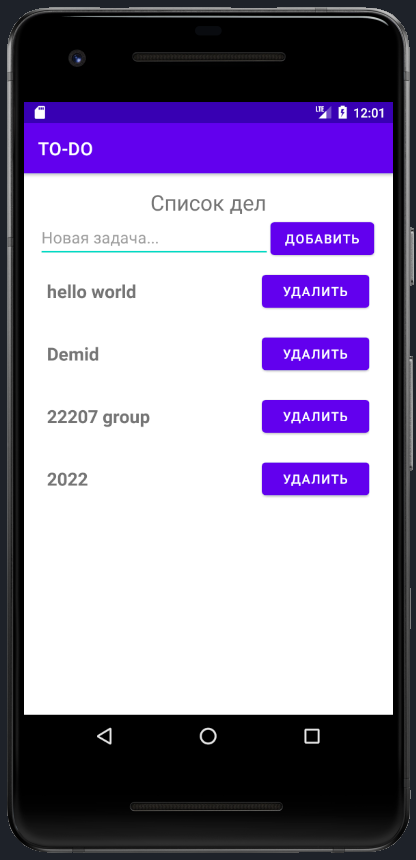
\includegraphics[scale=0.8]{images/todoapp.png}
\end{center}

%%%                          %%%
%%%%%%%%%%%%%%%%%%%%%%%%%%%%%%%%

%%%%%%%%%%%%%%%%%%%%%%%%%%%%%%%%
%%%                          %%%
%%% Приложение               %%%

\newpage
\appendix
%\section*{Приложение}
%\addcontentsline{toc}{section}{Приложение}
%\titleformat{\section}[display]
%  {\normalfont\Large\bfseries}
%  {Приложение\ \thesection}
%  {0pt}{\Large\centering}
%\renewcommand{\thesection}{\Asbuk{section}}

%%%                          %%%
%%%%%%%%%%%%%%%%%%%%%%%%%%%%%%%%
\end{document}

